\documentclass[usenames,dvipsnames]{standalone}
\usepackage{tikz}
\usetikzlibrary{shapes.geometric} % required for elliptical nodes
\usetikzlibrary{arrows.meta} % required for triangle arrow ends
\usepackage{xcolor}

\begin{document}
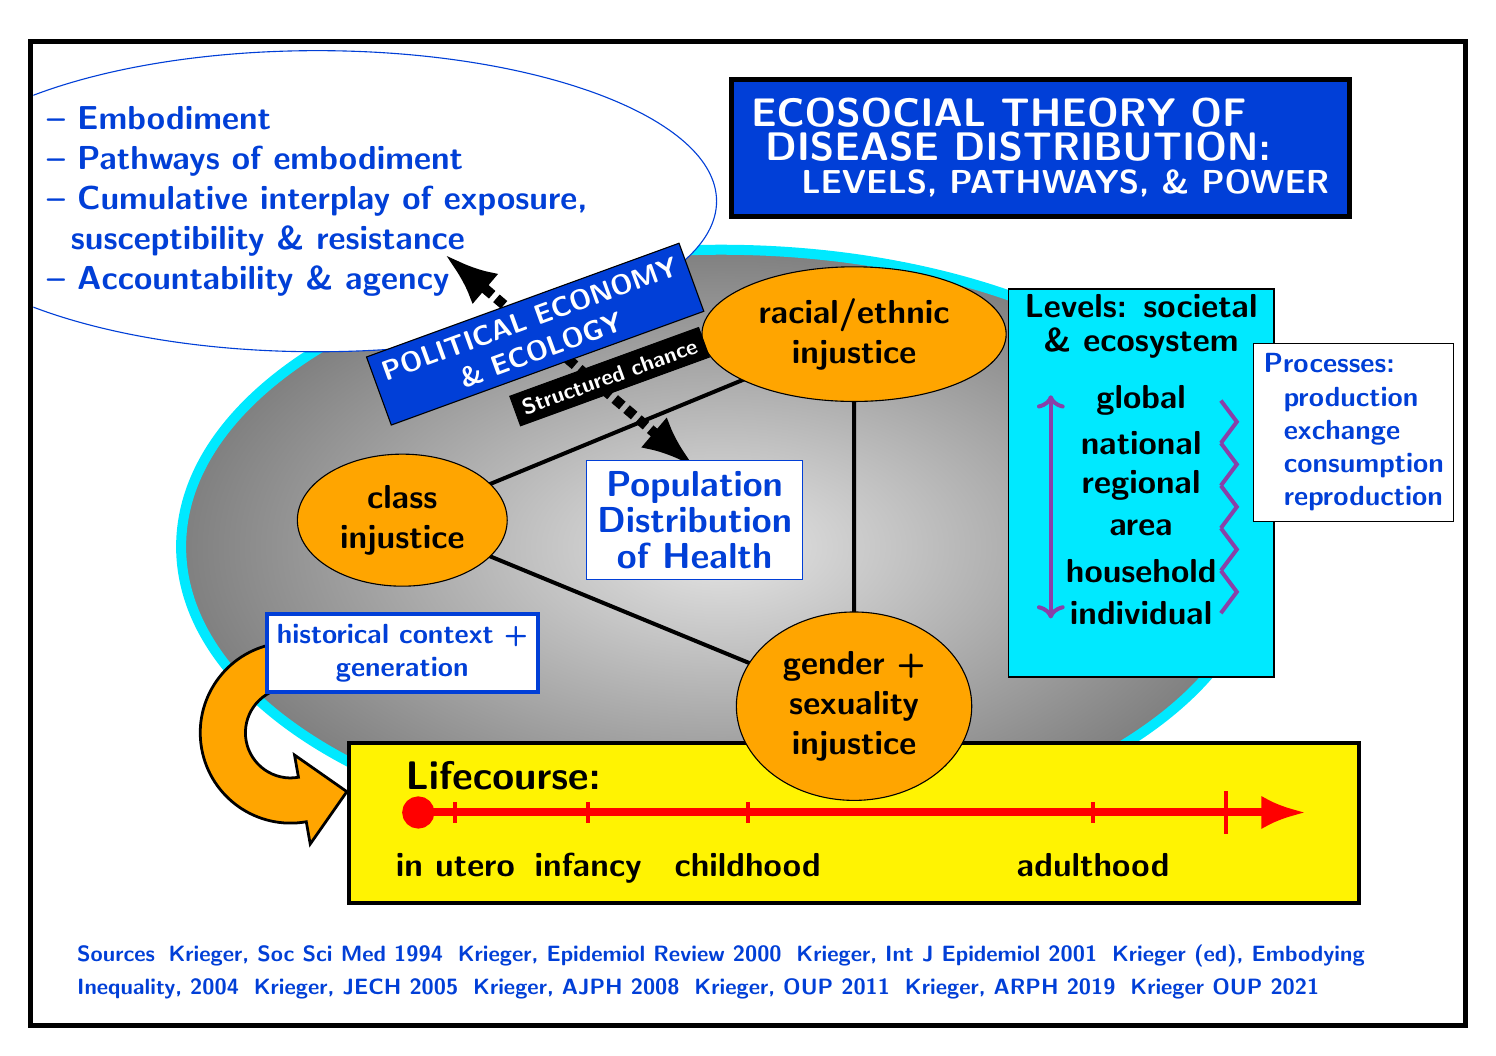
\begin{tikzpicture}[scale=1.35, outer sep=.1in, inner sep=.05in]

    % style
    \tikzset{font=\sffamily\bfseries};
    \definecolor{myblue1}{RGB}{1, 63, 215}
    \definecolor{myorange}{RGB}{255, 165, 0}
    \definecolor{myyellow}{RGB}{255, 243, 2}
    \definecolor{mypurple}{RGB}{136, 65, 168}
    \definecolor{mycyan}{RGB}{0, 233, 255}
    
    % empty elements to add padding at top, sides, and bottom
    \node [ellipse,fill=white] at (0,4.25) {\hspace{.25in}};
    \node [ellipse,fill=white] at (8.5,4.25) {\hspace{.25in}};
    \node [ellipse,fill=white] at (-2,4.25) {\hspace{.25in}};

    % background box for entire figure 
    \draw [draw=black, line width=.025in] (-3,4.25) rectangle (10.5,-5) {};

    % reference coordinates 
    \coordinate (Heading) at (6.5,3.25);
    \coordinate (EmbodimentOval) at (-.3,2.75);
    \coordinate (LevelsBoxCenter) at (7.45, .1);
    \coordinate (HealthCenter) at (3.5,0);
    
    % Heading
    \node [rectangle, fill=myblue1, line width=.025in, draw=black, text=white, align=left, inner sep = .1in] at (Heading) {\Large{ECOSOCIAL THEORY OF} \\ \Large{\hspace{.07in}DISEASE DISTRIBUTION:} \\ \hspace{.2in} \large{LEVELS, PATHWAYS, \& POWER}};

    % Background gray ellipse
    \draw [inner color=gray!20, outer color = gray] (3.5,-.5) ellipse (2in and 1.1in);
    \draw [draw=mycyan, line width=.05in] (3.5,-.5) ellipse (2in and 1.1in);

    % Lifecourse Timeline
    \filldraw [fill=myyellow, draw=black, line width = 0.02in] (0,-2.35) rectangle (9.5, -3.85); 
    \node at (1.45,-2.65) {\Large{Lifecourse:}};
    \draw [{Circle}-Latex, draw=red, line width=.04in] (.5,-3) -- (9,-3);
    \foreach \x/\xtext in {1/\large{in utero}, 2.25/\large{infancy}, 3.75/\large{childhood}, 7/\large{adulthood}}
    \draw [draw=red, line width = 0.02in] (\x,-2.9) -- (\x,-3.1) node [below] {\xtext};
    \draw [draw=red, line width = 0.02in] (8.25,-2.8) -- (8.25,-3.2);
    % fancy arrow from historical context + generation to Lifecourse
    \begin{scope}[xscale=-1]
    \tikzset{shift={(.55,-2.25)}, scale=.85}
    \draw[rotate=80,fill=myorange,line width=1pt] (-0:1cm) arc (0:-180:1cm) -- (-180:1.25cm) -- (-.75,.5) -- (-180:.25cm) -- (-180:.5cm) arc (-180:0:.5cm)--cycle;
    \end{scope}
    \node [text=myblue1, draw=myblue1, fill=white, align=center, line width = 0.02in] at (.5, -1.5) {historical context +\\generation};

    % Levels: Societal & ecosystem Hierarchy
    \filldraw [fill=mycyan, draw=black] ([shift=({-1.25,1.825})]LevelsBoxCenter) rectangle ([shift=({1.25,-1.825})]LevelsBoxCenter);
    % LevelsBoxCenter (6, 1.025)    
    \node [align=center] at ([shift=({0,1.475})]LevelsBoxCenter) {\large{Levels: societal}\\ \large{\& ecosystem}};
    \foreach \y/\ytext [remember=\y as \lasty (initially 1.8)] in {1.4/national, 1.0/regional, 0.6/area, 0.2/household, -0.2/individual}
    {
        \node at ([shift=({0,\y-1.025})]LevelsBoxCenter) {\large{\ytext}};
        \draw [draw=mypurple, line width = .02in] ([shift=({.75,\lasty-1.025})]LevelsBoxCenter) -- ([shift=({.9,\y-1.025+.2})]LevelsBoxCenter) -- ([shift=({.75,\y-1.025})]LevelsBoxCenter); % zigzag line
    }
    \node at ([shift=({0,.775})]LevelsBoxCenter) {\large{global}}; % first node is added separately to avoid the zigzag line
    \node[align=left, rectangle, text=myblue1, draw=black, fill = white, inner sep = .05in] at ([shift=({2,.475})]LevelsBoxCenter) {Processes:\\
    \hspace{.05in} production\\
    \hspace{.05in} exchange\\
    \hspace{.05in} consumption\\
    \hspace{.05in} reproduction
    };
    \draw [draw=mypurple, line width = .02in] [<->] ([shift=({-.85,-1.275})]LevelsBoxCenter) -- ([shift=({-.85,.825})]LevelsBoxCenter);

    % Left Hand Upper Corner Blurb on Embodiment, Pathways, etc. Accountability
    \begin{scope}
    \clip (-2.97, 4.25) rectangle (10,-5);
    \node[draw, ellipse, align=left, fill = white, draw=myblue1, text=myblue1, scale = 1.2] at (EmbodimentOval) { -- Embodiment\\ -- Pathways of embodiment\\ -- Cumulative interplay of exposure, \\ \hspace{.05in} susceptibility \& resistance\\ -- Accountability \& agency};
    \end{scope}

    % Injustice Relationships
    % triangle
    \draw [line width=.02in] ([shift=({1.25,1.5})]HealthCenter) -- ([shift=({1.25,-2})]HealthCenter) -- ([shift=({-3,-.25})]HealthCenter) -- cycle; % draw a triangle
    % labels for injustices 
    \node [ellipse, fill=myorange, draw=black, align=center, scale=1.2] at ([shift=({1.25,1.5})]HealthCenter) {racial/ethnic\\injustice};
    \node [ellipse, fill=myorange, draw=black, align=center, scale = 1.2] at ([shift=({1.25,-2})]HealthCenter) {gender +\\ sexuality\\injustice};
    \node [ellipse, fill=myorange, draw=black, align=center, scale = 1.2] at ([shift=({-3,-.25})]HealthCenter) {class\\injustice};
    % dotted arrow to embodiment
    \draw [Latex-Latex] [dotted, line width=0.05in] ([shift=({-.25,.25})]HealthCenter) -- ([shift=({1.2,-.5})]EmbodimentOval);
    % political economy ecology label
    %     \coordinate (HealthCenter) at (3.5,0);
    \node [draw=black, fill=myblue1, text=white, rotate = 20, align=center, scale=1] at ([shift=({-1.75,1.5})]HealthCenter) {POLITICAL ECONOMY \\ \& ECOLOGY};
    % structured chance 
    \node [draw=black, fill=black, text=white, rotate = 20, align=center, scale = .8] at ([shift=({-1.05,1.1})]HealthCenter) {Structured chance};

    % Population Distribution of Health
    \node[draw = myblue1, rectangle, fill = white, text=myblue1, scale=.75, scale=1.45, align=center] at ([shift=({-.25,-.25})]HealthCenter) {\large{Population}\\\large{Distribution}\\\large{of Health}};

    % footnotes
    \node [text=myblue1, align=left] at (3.5,-4.5) {\footnotesize{Sources\: Krieger, Soc Sci Med 1994\; Krieger, Epidemiol Review 2000\; Krieger, Int J Epidemiol 2001\; Krieger (ed), \textit{Embodying}}\\\footnotesize{\textit{Inequality}, 2004\; Krieger, JECH 2005\; Krieger, AJPH 2008\; Krieger, OUP 2011\; Krieger, ARPH 2019\; Krieger OUP 2021
    }};

\end{tikzpicture}
\end{document}
